%%%% CAPÍTULO 2 - REVISÃO DA LITERATURA (OU REVISÃO BIBLIOGRÁFICA, ESTADO DA ARTE, ESTADO DO CONHECIMENTO)
%%
%% O autor deve registrar seu conhecimento sobre a literatura básica do assunto, discutindo e comentando a informação já publicada.
%% A revisão deve ser apresentada, preferencialmente, em ordem cronológica e por blocos de assunto, procurando mostrar a evolução do tema.
%% Título e rótulo de capítulo (rótulos não devem conter caracteres especiais, acentuados ou cedilha)
\chapter{Fundamentação te\'orica}\label{cap:referencialTeorico}

Neste capítulo são apresentados alguns conceitos importantes para o entendimento
do trabalho, sendo abordados assuntos como biometria, processamento de imagens, aprendizado 
profundo e reconhecimento facial.

\section{Microcontrolador}\label{sec:microcontrolador}

Microcontrolador é um computador em um único \textit{chip} que incorpora: processador, 
memória, periféricos de entrada e saída, temporizadores e dispositivos de 
comunicação serial. Eles surgiram como uma evolução natural dos circuitos digitais 
devido à crescente complexidade. Chegou um ponto em que foi mais prático e 
econômico substituir a lógica das portas digitais por um conjunto de 
processador e \textit{software} \cite{penido2013}.

O primeiro microcontrolador, o ''8048'', foi lançado pela Intel em 1977 e evoluiu 
para a família ''8051''. Esses \textit{chips} são programados em linguagem \textit{Assembly} e 
possuem um conjunto de instruções poderoso \cite{penido2013}.

Atualmente, quando se trata de microcontrolador, uma boa opção é o ESP32 (\autoref{fig:esp32}). Mesmo não 
sendo o modelo mais potente, nem o mais compacto, ainda assim, possui um ótimo 
custo-benefício, considerando sua simplicidade, poder de processamento e baixo consumo 
de corrente \cite{espressif2022c}.

\begin{figure}[h!]
    \centering
    \caption{ESP32-DevKitC.}
    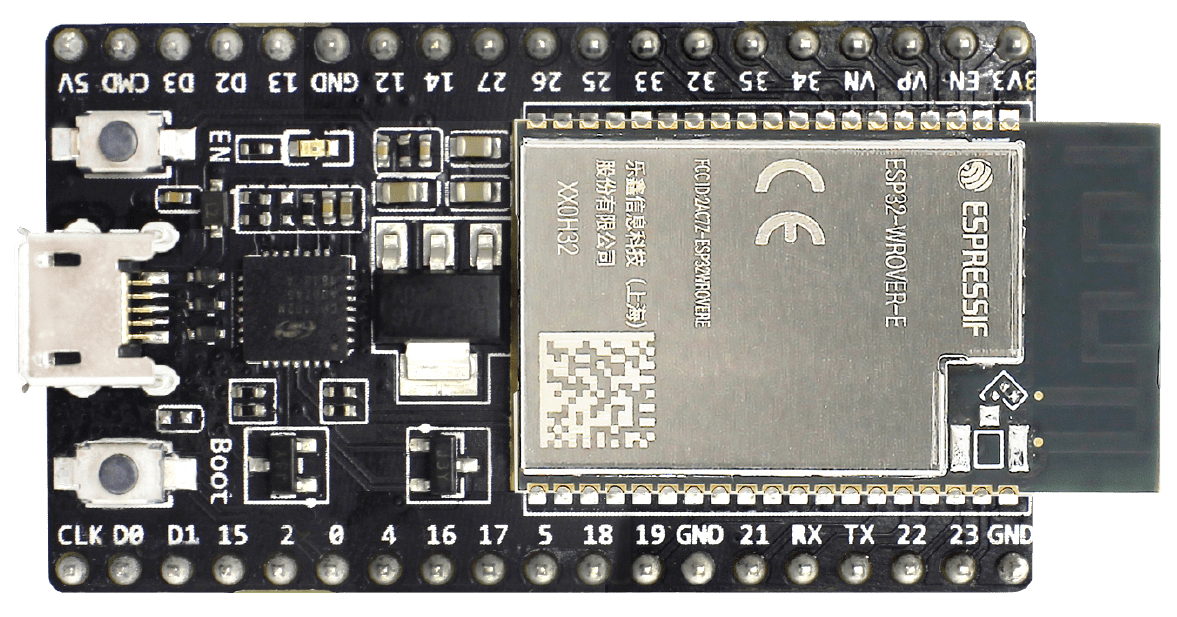
\includegraphics[scale=0.13]{figuras/esp323.png} 
    \legend{Fonte: Adaptado de \citeonline{espressifimg}.}
    \label{fig:esp32}
    \centering
\end{figure}

\section{Processamento de imagem}\label{sec:processamento}

As técnicas de processamento de imagens começaram a surgir no final da década de 1960, 
para serem utilizadas no realce e restauração de imagens capturadas do espaço, 
como por exemplo, as imagens da missão Apollo. Logo em seguida, essa tecnologia 
começou a ser empregada para processar imagens em diagnósticos médicos e, com 
o aumento do poder de processamento dos computadores, essas técnicas agora 
são empregadas nas mais diversas áreas de conhecimento \cite{gonzalez2010}.

Em processamento de imagens, um conceito bastante utilizado é a binarização de
imagens, que consiste em duas classes distintas, o fundo e o objeto, esse processo 
serve para separar ambas as classes.

Sendo assim, a forma mais simples de processamento consiste na
bipartição do histograma, dando valores iguais a 0 (branco) aos \textit{pixels} que estiverem
abaixo do valor de \textit{threshold} (T) e iguais a 255 (preto) aos \textit{pixels} que estiverem 
acima desse valor. Na \autoref{fig:escalacinza} é possível observar uma escala de 
tons de cinza e na \autoref{fig:escalabinarizada} verifica-se essa mesma escala 
pós-processamento, exemplificando o processo de binarização.

\begin{figure}[h!]
    \centering
    \caption{Escala de cinza}
    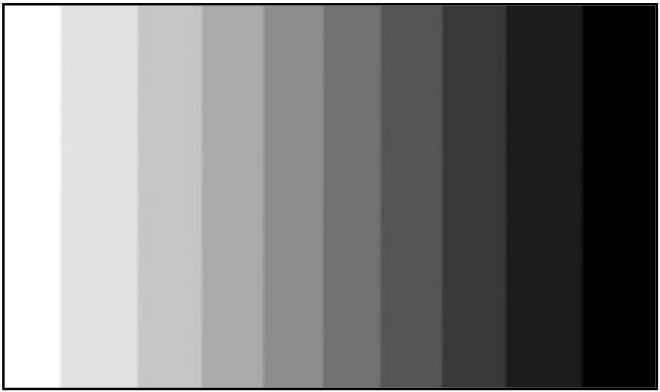
\includegraphics[scale=0.25]{figuras/escala_cinza.png} 
    \fonte{}%% Fonte
    \label{fig:escalacinza}
    \centering
\end{figure}

\begin{figure}[h!]
    \centering
    \caption{Escala de cinza binarizada}
    
\includegraphics[scale=0.25]{figuras/escala_binarizada.png} 
    \fonte{}%% Fonte
    \label{fig:escalabinarizada}
    \centering
\end{figure}

Especialmente durante o processo de reconhecimento de objetos, 
a segmentação é uma ferramenta indispensável para fins de análise e interpretação.

A segmentação de uma imagem é um procedimento importante no que tange
essas análises, uma vez que ela subdivide uma imagem em regiões que
posteriormente serão ou não tidas como de interesse, o que pode variar muito de
acordo com a aplicação \cite{gonzalez2010}.

Os principais algoritmos de segmentação de imagem têm suas bases em duas 
abordagens: descontinuidade e similaridade. A abordagem da descontinuidade 
envolve a divisão de uma imagem com base em mudanças abruptas de 
intensidade, como as que ocorrem nas bordas. Por outro lado, a técnica 
de similaridade segmenta a imagem com base na identificação de regiões 
que compartilham semelhanças de acordo com critérios 
predefinidos \cite{gonzalez2010}.

Por fim, uma outra técnica conhecida como esqueletização, 
consiste na representação de um conjunto de pontos no interior de um 
objeto de uma imagem. O esqueleto de uma região pode
ser definido pela transformada do eixo médio (MAT) do inglês (\textit{medial axis
transformation}). Nessa técnica, são selecionados os elementos centrais de um objeto,
criando literalmente um esqueleto da imagem. MAT de uma região \textit{R} com uma borda
\textit{B} é definida como: para cada ponto \textit{p} contido na região, encontramos seu vizinho
mais próximo em \textit{B} (borda), e se houver mais de um vizinho então o ponto pertence
ao eixo médio, ou seja, ao esqueleto \cite{gonzalez2010}.

O que pode ser visualizado com mais facilidade na \autoref{fig:esqueletizacao}:

\begin{figure}[h!]
    \centering
    \caption{Processo de esqueletização}
    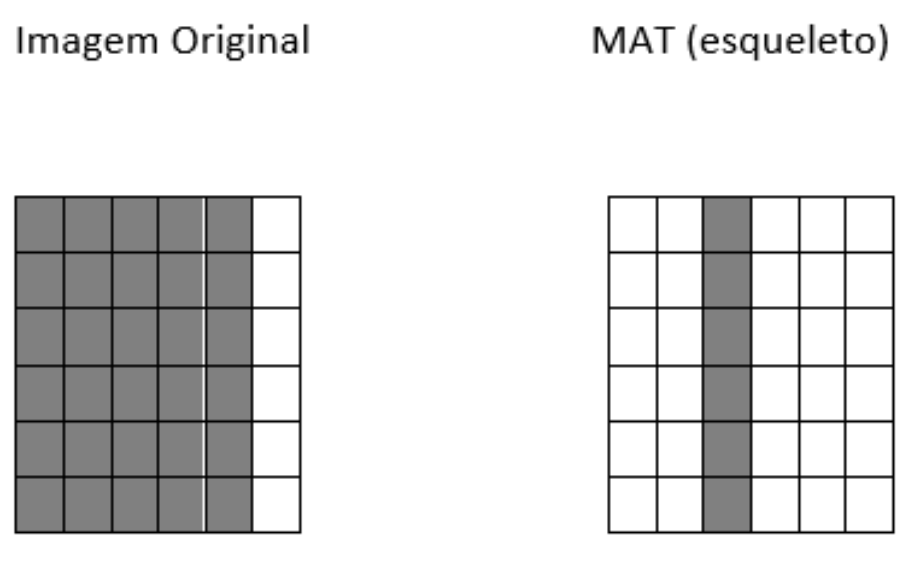
\includegraphics[scale=0.25]{figuras/esqueletizacao.png} 
    \fonte{}%% Fonte
    \label{fig:esqueletizacao}
    \centering
\end{figure}

\section{Biometria}\label{sec:biometria}

Com o avanço da tecnologia, hoje é possível realizar transações e pagamentos 
de qualquer lugar, ou até mesmo, sem sair de casa, apenas com o uso de 
um dispositivo conectado a internet. Entretanto, também tornaram-se indispensáveis 
o uso de mecanismos de segurança, principalmente os que são capazes de identificar 
e comprovar quem realmente está utilizando esses serviços.

Por mais que existam outros processos de identificação, como por exemplo, cartões 
magnéticos, senhas, tags, etc., atualmente o processo considerado mais seguro é 
o baseado em biometria.

A biometria pode ser definida como o processo de identificação 
dos seres vivos e tem por intuito distinguir os indivíduos por meio 
de suas características únicas. É uma técnica que foi utilizada até mesmo pelos egípcios 
para o processo de identificação, baseando-se em características da
aparência dos indivíduos, como cor dos olhos e cicatrizes \cite{santos2007}.

Os sistemas biométricos podem ser divididos em dois grupos distintos: 
1) os métodos invasivos, que requerem a colaboração ativa do sujeito 
para a identificação; e 2) os métodos não invasivos, que podem ser 
aplicados sem que o indivíduo identificado tenha conhecimento disso. 
Entre os métodos, incluem-se técnicas amplamente conhecidas, 
como a biometria da impressão digital, do rosto, da íris, da assinatura, 
entre outras \cite{teixeira2011}

O foco deste estudo será um método de biometria não invasivo, mais 
precisamente no processo de identificação e reconhecimento de 
características faciais, um tema que tem atraído crescente 
interesse de pesquisadores e cientistas na área de visão 
computacional.

\section{História da biometria}\label{sec:histbiometria}

Contrariando o senso comum, é importante notar que o conceito de biometria 
não é algo recente, o que realmente se tornou inédito foi a sua aplicação 
em sistemas computacionais. Na verdade, práticas de identificação com base 
em características físicas datam de muito tempo atrás. Um exemplo notório 
é o uso que os faraós do Egito faziam de características como cicatrizes, 
cor dos olhos, arcada dentária e outros detalhes para distinguir 
indivíduos \cite{boechat2008}.

Na Europa, por volta de 1890, o antropologista e delegado policial 
parisiense Alphonse Bertillon viu na biometria uma maneira de identificar 
criminosos e a transformou em uma nova área de estudo \cite{moraes2006}. 
Bertillon, com um profundo interesse em pesquisas criminalísticas, 
começou a medir diversas partes do corpo humano, incluindo o diâmetro 
transversal da cabeça, comprimento dos pés, dedos, antebraços, estatura, 
entre outros e, registrou essas medidas em cartões. Embora os resultados 
obtidos por Bertillon não tenham sido conclusivos, a ideia de relacionar 
medidas do corpo humano para a identificação continuou a ser usada 
por autoridades policiais em todo o mundo, sendo conhecida como 
''Bertillonage'' \cite{boechat2008}.

Na \autoref{fig:bertillon}, podem ser observadas várias técnicas de medição 
desenvolvidas por meio do método de Bertillon, abrangendo aferições dos 
braços, pernas, cabeça e até mesmo das orelhas.

\begin{figure}[h!]
    \centering
    \caption{Método de Bertillon}
    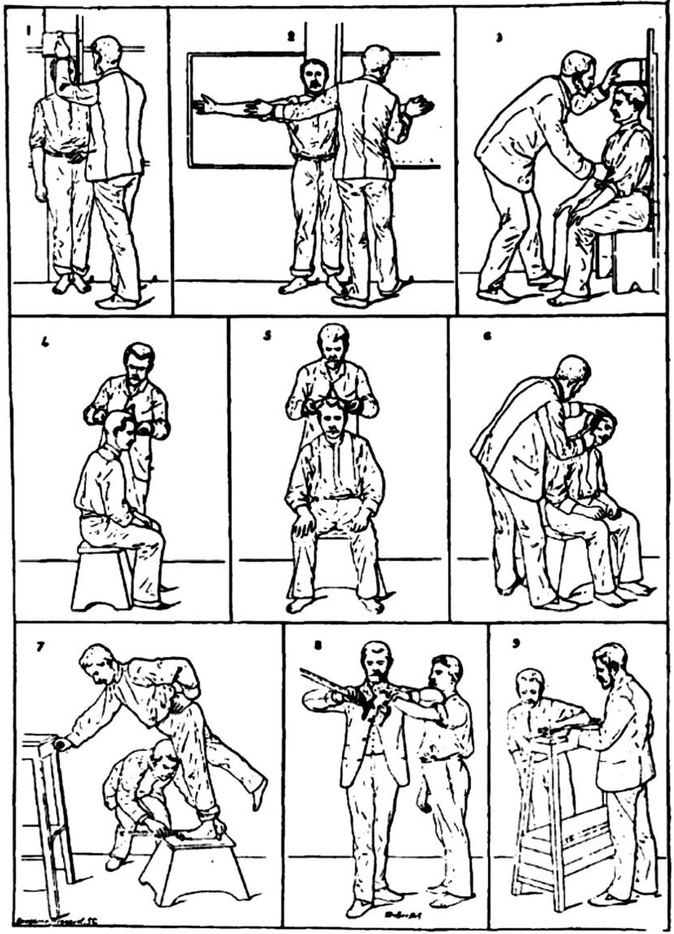
\includegraphics[scale=0.25]{figuras/bertillon.jpg} 
    \legend{Fonte: Adaptado de \cite{moraes2006}.}
    \label{fig:bertillon}
    \centering
\end{figure}

Na Suíça, com a introdução da fotografia, essa técnica começou a ser 
usada de maneira exclusiva nos procedimentos de identificação 
criminal. Na Índia, um indivíduo chamado William James Hersche, 
insatisfeito com a falta de cumprimento de contratos por parte 
dos comerciantes locais, passou a exigir que as assinaturas 
fossem acompanhadas pela impressão digital nos documentos \cite{boechat2008}.

Por fim, nas últimas décadas, novos sistemas biométricos começaram a surgir 
à medida que novas aplicações biométricas eram desenvolvidas e se tornavam 
uma realidade comercial.

\section{Tipos de biometria}\label{sec:tiposBiometria}

De acordo com \citeonline{morais2010}, os principais tipos de biometria são:

\begin{itemize}
    \item Orelhas: usa a anatomia da orelha para identificar indivíduos, abordagem 
    incomum. 

    \item Termograma da face e das mãos: o padrão de calor emitido pelo corpo 
    humano é uma característica de cada pessoa e pode ser captado por 
    infravermelho. Sistemas baseados em imagens termográficas não requerem 
    contato ou cooperação individual. No entanto, a captura de imagem continua 
    sendo um desafio em ambientes não controlados, pois é afetada por fontes de 
    calor que possivelmente podem estar próximas ao indivíduo. Seus pontos fortes 
    são a universalidade, a impostura e a singularidade.

    \item Impressão digital: como pode ser observado na \autoref{fig:digital}, 
    recurso mais comumente usado em credenciais 
     automatizadas em grande escala.  Sua popularidade se deve em parte a 
     dispositivos de coleta de baixo custo e desempenho de processo razoável. 
     Embora a impressão digital não se modifique naturalmente ao longo dos anos, 
     ela é sensível aos fatores ambientais aos quais os indivíduos estão 
     submetidos, o que pode levar à sua alteração e deterioração. Trabalhadores 
     manuais, por exemplo, podem ver suas impressões digitais constantemente 
     alteradas devido a cortes profundos ou outros cortes em seus dedos.
     
     \begin{figure}[h!]
        \centering
        \caption{Modelo de impressão digital}
        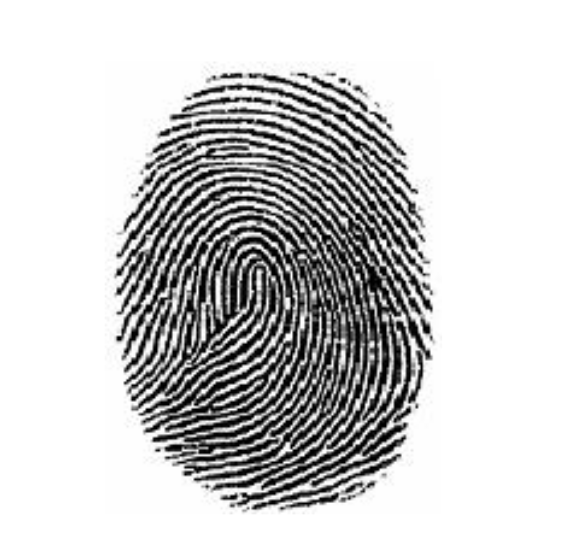
\includegraphics[scale=0.2]{figuras/impressao_digital.png} 
        \legend{Fonte: Adaptado de \cite{boechat2008}.}
        \label{fig:digital}
        \centering
    \end{figure}

    \item Íris: formada durante o desenvolvimento fetal, estabiliza-se durante 
    os dois primeiros anos de vida. Sua textura é extremamente complexa e 
    fornece informações a serem utilizadas no reconhecimento facial. Tem um baixo grau 
    de impostura, pois é difícil até cirurgicamente alterar a textura da íris. 
    Seu ponto fraco está em sua capacidade de recuperação, requer equipamentos 
    caros e complexos, bem como cooperação individual.

    \item Voz: união de biometria comportamental e fisiológica. Ele não muda 
    em curtos períodos de tempo, mas é afetado por fatores como um simples frio, 
    estado emocional e ruído de fundo. Possui baixa exclusividade e não é 
    recomendado para identificação em larga escala. O ponto forte é a capacidade 
    de coleta e aceitabilidade, além do baixo custo dos coletores. Geralmente 
    indicado para verificação de identidade em conversas.
\end{itemize}

\section{Reconhecimento facial}\label{sec:reconhecimento}

Desde a infância, o ser humano adquire e desenvolve sua capacidade de reconhecer traços faciais, 
que é uma particularidade da visão e fundamental para relações sociais \cite{rouhani2019}.

Existem estudos sobre automatização do reconhecimento facial desde os anos 60. Os projetos iniciais nessa 
área dependiam do administrador encontrar manualmente as características faciais nas imagens, só 
então o sistema calculava as distâncias entre elas e comparava suas dimensões normalizadas com 
as referenciadas.

O processo de reconhecimento facial pode ser descrito a partir de uma imagem ou vídeo estático, 
identificando um ou múltiplos indivíduos a partir de um banco de dados de rostos previamente 
cadastrados. Assim, existem três abordagens conhecidas para reconhecimento:

\begin{itemize}
    \item Imagem a imagem: a amostra e a base de dados composta por imagens estáticas;

    \item Vídeo para vídeo: a amostra e o banco de dados que consiste em vídeos;

    \item Imagem para vídeo: o exemplo é um vídeo. O vídeo é comparado a um banco de 
    dados de imagens estáticos. 
\end{itemize}

Após a imagem ter sido lida e transformada, a mesma é duplicada e redimensionada 
proporcionalmente para uma altura fixa. A imagem original é mantida para ser 
utilizada posteriormente. Em seguida, a imagem é convertida para escalas de 
cinza e então equalizada para realçar o contraste e facilitar a detecção de faces.

A seguir, é feita a detecção das faces utilizando o classificador 
de objetos treinados. Removendo o fundo ao redor da face, pois 
pode atrapalhar os algoritmos de reconhecimento.

As abordagens mais populares usadas no problema de reconhecimento facial são 
baseadas na localização e análise de atributos faciais como olhos, nariz e 
boca (\autoref{fig:haarcascate}), ou em análise global destes.

\begin{figure}[h!]
    \centering
    \caption{Reconhecimento baseado na localização dos olhos e nariz}
    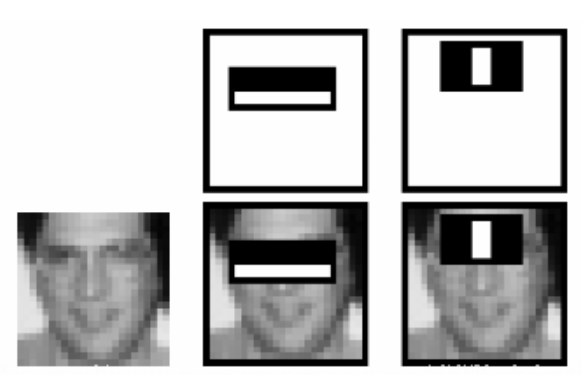
\includegraphics[scale=0.35]{figuras/haarcascate.png}
    \legend{Fonte: Adaptado de \citeonline{viola2004}.}
    \label{fig:haarcascate}
    \centering
\end{figure}

Ao comparar as informações extraídas com aquelas já conhecidas, 
complementadas por uma breve análise estatística, é possível 
categorizar o objeto e determinar com grande precisão sua natureza 
ou identidade \cite{gonzalez2010}.

\section{Biometria facial para controle de acesso}\label{sec:biometriaFacial}

Os sistemas de identificação baseados em biometria são essencialmente sistemas de 
reconhecimento que, dadas informações biométricas, são capazes de distinguir padrões e 
classificá-los em diferentes classes ou categorias \cite{morais2010}.

Ainda de acordo com o autor, algumas das principais características anatômicas, 
fisiológicas e comportamentais utilizadas em sistemas biométricos incluem 
impressão digital, impressão da mão, aparência facial, temperatura da face, 
retina, voz, assinatura, entre outras.

A biometria facial representa a técnica biométrica mais adotada atualmente. 
Embora o reconhecimento de rostos seja uma tarefa simples para as 
pessoas, ela se revela notavelmente complexa para os computadores. 
Mesmo em condições desafiadoras, o cérebro humano é capaz de identificar 
com precisão uma pessoa com base em sua imagem facial, apesar das variações 
na iluminação, distorções ou deformações.

Embora os sistemas biométricos faciais apresentem um desempenho aceitável em 
ambientes comerciais, ainda estão sujeitos a restrições relacionadas ao ambiente, 
como variações na iluminação (\autoref{fig:iluminacao}) e ângulos das imagens.
Segundo \citeonline{cavalcanti2005}, alterações estéticas, como cabelo e barba, uso de
acessórios, como óculos e bonés, são fatores que aumentam as chances de falha no processo
de reconhecimento facial.

\begin{figure}[h!]
    \centering
    \caption{Rostos em diferentes iluminações}
    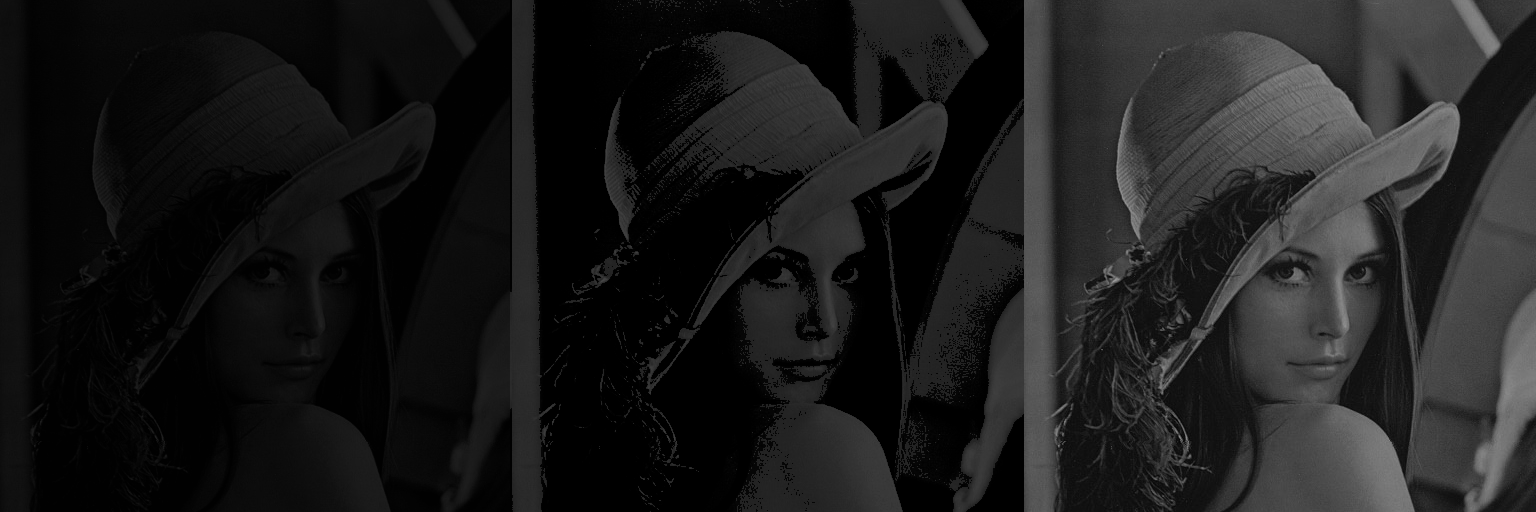
\includegraphics[scale=0.25]{figuras/iluminacao.png}
    \legend{Fonte: Adaptado de \citeonline{opencv4}.}
    \label{fig:iluminacao}
    \centering
\end{figure}

Para utilizar a face em sistemas biométricos é preciso seguir três
etapas fundamentais. São elas:

\begin{itemize}
    \item Detecção facial: responsável por definir e localizar uma ou mais
    faces;

    \item Extração de características: esta fase é responsável por remover o excesso de
    informações que rodeiam as faces detectadas, assim como selecionar as melhores
    características para serem utilizadas na próxima etapa;

    \item Reconhecimento facial: esta fase compara as características selecionadas pela fase
    anterior com outras previamente cadastradas em um banco de dados, sendo
    responsável por encontrar um registro que se assemelhe ao que precisa ser
    identificado.

\end{itemize}

Essas etapas desempenham um papel fundamental na avaliação da imagem, eliminando informações 
redundantes e irrelevantes. Por exemplo, se o algoritmo identifica uma ou mais faces na 
imagem, essas são extraídas da imagem original para análise individual. É importante 
notar que, quando a entrada do sistema é uma sequência de vídeo, a dimensão temporal 
também é considerada, tornando essencial que o algoritmo opere em tempo real, com 
desempenho crítico, para permitir a detecção em tempo real \cite{boechat2008}. 

Muitos algoritmos de detecção facial requerem treinamento para produzir resultados 
satisfatórios. Esse treinamento envolve o uso de diversas imagens de faces 
e objetos diferentes.

Os algoritmos de reconhecimento facial têm a capacidade de identificar indivíduos com 
base em características específicas, como o tamanho dos olhos, nariz e boca. Essas 
características são usadas para localizar imagens correspondentes que se assemelham 
à imagem da face capturada. Além disso, os algoritmos desse tipo normalmente armazenam 
informações relevantes apenas da região da imagem que contém as características de 
interesse, conforme pode ser observado na \autoref{fig:facereg}. De acordo 
com \cite{brunelli1993}, um dos primeiros sistemas de reconhecimento 
facial baseava-se em um modelo de técnicas aplicadas a um conjunto de características 
faciais, resultando em uma representação facial compacta e correspondente.

\begin{figure}[h!]
    \centering
    \caption{Pontos de referência a partir de características faciais}
    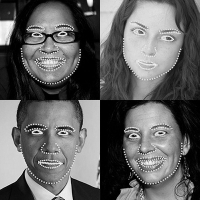
\includegraphics[scale=0.9]{figuras/facereg.jpg}
    \legend{Fonte: Adaptado de \citeonline{opencv5}.}
    \label{fig:facereg}
    \centering
\end{figure}